\documentclass{article}
\usepackage{graphicx}
\usepackage{tabulary}
\usepackage{caption}
\usepackage{xeCJK}
\setCJKmainfont{AR PL UKai CN}

\title{性能测试报告}  
\author{wuziheng}

\begin{document}
\maketitle
\section{流程分析}关于检测速度,我们需要将整个问题的流程进行详细的分析。对于一帧测试图像整个过程大致分为如下图
	\begin{figure}[ht]

	\centering
	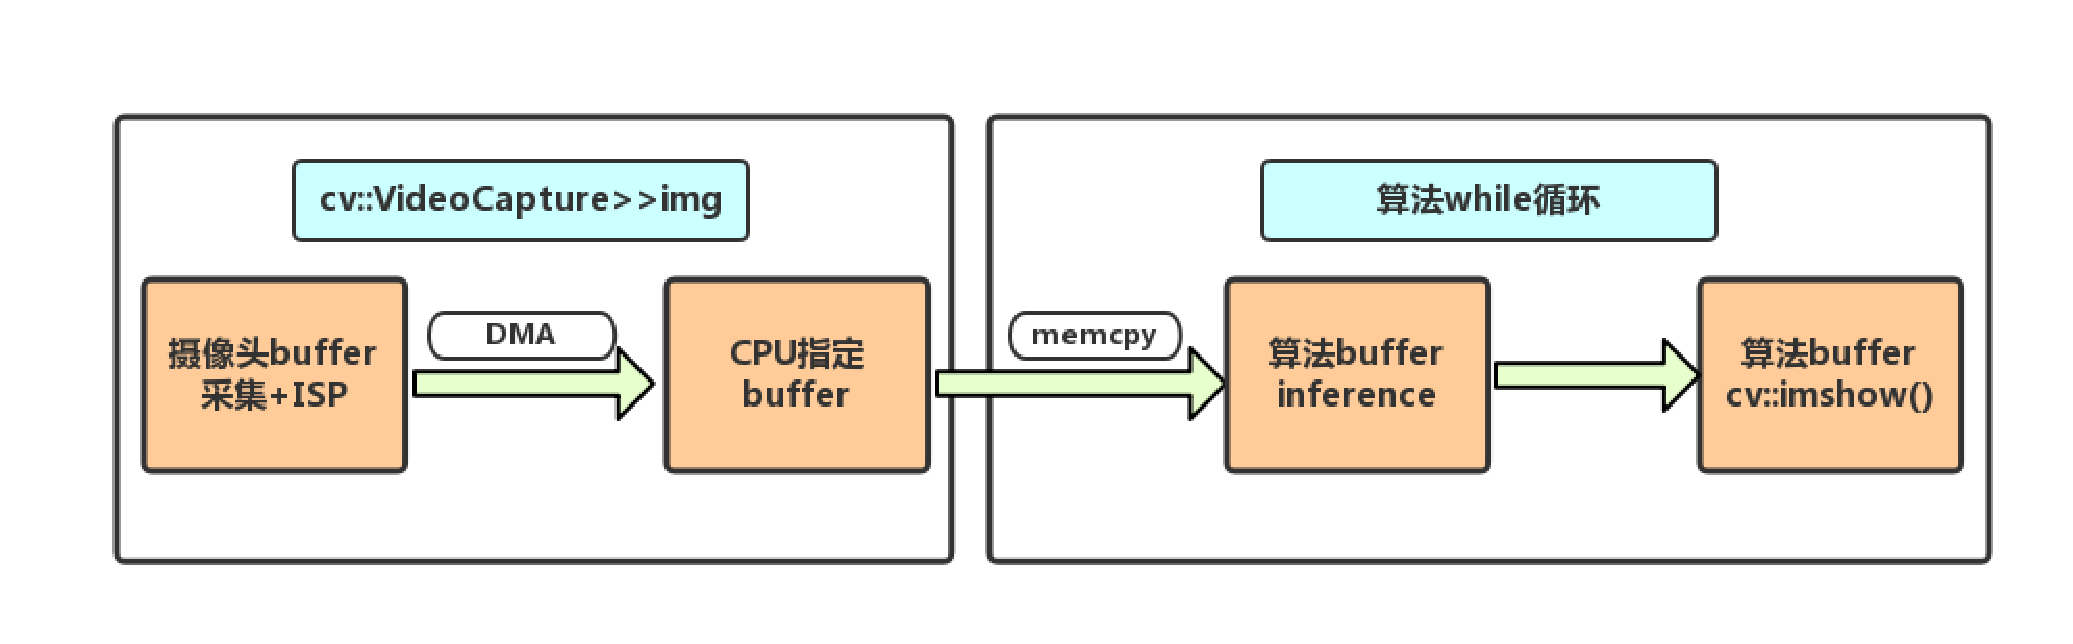
\includegraphics[scale=0.35]{pic/isp.eps}
	\caption{主要流程分析}
	\label{fig:label}
	\end{figure}

	\begin{itemize}
	\item 摄像头负责采集并做ISP等功能的时间由摄像头规格决定(包括曝光时间,处理速度等等)
	\item DMA时间由带宽决定,而由cpu拷贝至算法指定的buffer的时间由Opencv算法的实现和cpu性能决定
	\end{itemize}

\paragraph{}上述这一部分在比赛中限定使用cv::VideoCapture() >> img 实现,笔者关闭了整个算法循环的内容,可以测出cv::VideoCapture>>img的速度约为25fps,即该摄像头规格为480p25.实际在使用中,如果算法while循环一次的时间小于40ms,则需要继续等待下一帧img通过memcpy传输过来。

\paragraph{}当然笔者也进行了测试,在该平台上cv::imshow()一帧480p的图像平均时间在10到13ms之间。在这个情况下,会显示cap>>img的时间约为(40-13)=27ms左右。进一步的测试总结如下表格:

	\begin{table}[h]
		\centering
  		\begin{tabulary}{1.2\textwidth}{CCCCC}
  		主要流程 & ISP+Capture  & memcpy & cv::imshow & inference \\
    	\hline
		 time  & 40ms & 12ms(uncertain )& 10 \~ 13ms & 3 \~ 5ms \\
  		\end{tabulary}  
  		\caption{流程时间测试}
		\label{tab:Margin_settings}
	\end{table}

\paragraph{}到这里我们也就理清了cv::VideoCapture的工作原理(应该是算法线程会去开辟一个新的现成去完成左边框内的工作)。而算法线程每一帧图像在副线程完成DMA之后,就会拷贝给算法开辟的buffer中去,这个间隔是40ms。也就是说如果memcpy+inference+cv::imshow()的时间小于40ms,这个时候在算法线程就会挂起等待DMA结束。


\paragraph{\emph{Summary}}在Firefly-3399上,调用cv::VideoCapture作为采集,cv::imshow()作为显示,如果你的inference时间小于15ms(40-13-12)每帧,那么多余的速度将不会起到任何增益。例如笔者这里的inference在没有目标的时候大概是1ms,出现很大目标时是7到10ms,这样的波动根本不会影响实际帧率,因为算法永远会挂起等待DMA。考虑在实际的整个系统的流水线取决于最慢的一级,而摄像头一般都有最低的曝光和ISP处理时间,而这个时间将成为整个系统的瓶颈,也就是说在我们的板子上,最快显示出来的实际fps就是25,想要提升只能加速摄像头采集,提升规格。所以再优化检测算法的速度(inference)在现阶段也只有理论上的意义了。

\section{Inference性能测试}有了上面的讨论,这里我们就可以进入对检测算法的性能测评(以下对应每个手势的时间代表的是这个算法检出为某个手势的时间,是包括定位和分类一起的时间。而不是单独测试某一个分类器的时间):
	\begin{figure}[H]

	\centering
	\includegraphics[width=10cm,height=7cm]{pic/single.png}
	\caption{单手势检出时间}
	\label{fig:label}
	\paragraph{图例}蓝色:全局版 橙色:比赛版
	\end{figure}
		
	\begin{table}[htb]
		\centering
  		\begin{tabulary}{0.95\textwidth}{CCCCCCC}
  		dis=1.5m & no target& hearta&heartb&greet&six&thumb \\
    	\hline
		 time  & 0.7ms & 2.5ms & 3.5ms & 2.5ms & 4.9ms & 2.2ms\\
  		\end{tabulary}  
  		\caption{比赛版本 Single-Gestures Test}
		\label{tab:Margin_settings}
	\end{table}	
	

	\begin{table}[htb]
		\centering
  		\begin{tabulary}{0.95\textwidth}{CCCCCCC}
  		dis=1.5m & no target& hearta&heartb&greet&six&thumb \\
    	\hline
		 time  & 2.0ms & 3.3ms & 4.8ms & 2.8ms & 6.0ms & 3.5ms\\
  		\end{tabulary}  
  		\caption{全局版本 Single-Gestures Test}
		\label{tab:Margin_settings}
	\end{table}	
	


	\begin{figure}[htb]

	\centering
	\includegraphics[width=10cm,height=7cm]{pic/Muti.png}
	\caption{多手势检出时间}
	\label{fig:label}
	\paragraph{图例}蓝色:全局版 橙色:比赛版
	\end{figure}
	
	\begin{table}[htb]
		\centering
  		\begin{tabulary}{0.95\textwidth}{CCCCCCC}
  		dis=1.5m & 3six& 2hearta&2heartb&2greet&2six&2thumb \\
    	\hline 
		 time  & 10.3ms & 4.2ms & 8.1ms & 3.8ms & 6.8ms & 4.0ms\\
  		\end{tabulary}  
  		\caption{比赛版本 Muti-Gestures Test}
		\label{tab:Margin_settings}
	\end{table}
	
	\begin{table}[htb]
		\centering
  		\begin{tabulary}{0.95\textwidth}{CCCCCCC}
  		dis=1.5m & 3six& 2hearta&2heartb&2greet&2six&2thumb \\
    	\hline 
		 time  & 10.5ms & 8.3ms & 14.4ms & 3.3ms & 6.0ms & 4.1ms\\
  		\end{tabulary}  
  		\caption{全局版本 Muti-Gestures Test}
		\label{tab:Margin_settings}
	\end{table}


\newpage
\paragraph{\emph{PS:}}
	\begin{itemize}
	\item[1] 测试距离为1到1.5m,这个距离决定了vj搜索的最小框与最大框的参数,会对速度产生一定影响,可以根据需求修改,但是不要太远。对于太小的目标而言,算法框架可能需要精细的调整。(其实也很简单,可以咨询我694790961@qq.com)
	\item[2] 手势速度差距来源于手势训练处的xml的深度和每一层的弱分类器个数,总的来说,在训练分类器的过程里,还是要以recall和precision为关注点,训练出来可以用的再考虑在这一部分提升速度。
	\item[3] 以上的度比赛版本是在每3帧才全局搜索一次而其余两帧只做近邻搜索分类的情况下做的。全局版则是在每一帧都做全局搜索的情况下的测试结果
	\item[4] 对比结果发现,在预处理的时间上,比赛版有优势,但是在Viola-jones的时间上,全局版有优势。随着每一帧画面中手势数量的增多,Viola-jones的时间几乎是线性增加的,而预处理时间几乎不会变化,所以说在Muti-Gesture的应用场景里,我们推荐 frame\_ control=1,2,而在确定只有Single-Gesture的场景中,选择  frame\_control=3。比赛情况为后者。
	\item[5] 全局版会出现少量的误检,而比赛版则不会,因为 frame\_control 还控制了算法逻辑框架的其他部分可以消除大部分误检测。这也是选择比赛版的原因之一。
	\item[6] 算法还保留了利用 CNN 对检出的手势框进行再确认的接口,本意是用来提高precision,但是后期笔者解决了 precision 的问题,并且 CNN 较慢而且 recall 很低,会导致检出的手势也会被误判为背景,所以在比赛版本里关闭了 CNN 测试的接口。CNN在板子上的性能大约为10ms一个候选框。
	\item[7] 关于核心使用的问题,程序是默认使用6个核心,笔者的测试结果也表示默认是最快的,可能会有不同的结果。
	\end{itemize}

\end{document}